
\chapter{仮説検定の3つの枠組み}
現在利用されている仮説検定の枠組みを紹介する。
それぞれの枠組みは前提が異なっており、それぞれの問題で良い推測を与える。
適切な枠組みを選ばなければ間違った解釈をしてしまう事になる。
我々の行なっている科学では、F型の枠組みを使う。
以降の章では、F型の問題について考える。

\section{F型}
\subsection{解決できる問題}


\subsection{データとモデルの比較}
ここで、いくつかのことを定義しておく。
\begin{defi}
    統計モデルと標本を比較して、モデルが母集団のことを予測できないとさまざまな指標をもとに判断するとき、統計モデルを却下すると宣言する。
    %ある標本から求められた統計量以上に大きな値が得られる確率を$p$値と呼ぶ。
    %絶対にダメと判断されないときは、統計モデルを採択(棄却の対義語)すると宣言しない。
    %統計モデルが棄却されるのは、統計モデルの仮定によって変化する。本書の範囲内であれば、統計モデルの母数、分布関数、独立同一の分布関数からサンプリングされたことによる。
    %最尤統計モデルにおいて、棄却されない統計モデルの母数の範囲を信頼区間といい、棄却されるモデルの母数の範囲を棄却域という。
\end{defi}
%ある閾値$\alpha$を決めて、それよりも小さな$p$値をもつ標本について、モデルから得られたものではないと判断する。ここで、$\alpha$を有意水準という。

ここで、母集団から無作為抽出した標本(モデルから生成された標本ではない)を正規モデルにより、予測できるかを考える。
上記の議論と同様に、標本から、統計モデルにあった統計量を計算し、統計量よりも偏った値が出現する確率($p$値)を計算する。
$p$値が小さければ、モデルにより予測できないと考え、値が1に近いほど、もしかしたらモデルで予測できるのかもしれないと考える\footnote{$p$値だけで判断してはいけない}。
標本を元に、モデルにより予測ができないかを考えている。
%このとき、モデルを却下すると宣言する。
%$p$値が$\alpha$よりも小さいとき、流石にこのモデルでは予測できないでしょうと判定する。
%$p$値が$\alpha$よりも大きい場合でも、そのままこのモデルで予測できるとは宣言しない。他の指標やデータとモデルをグラフにより比較し、予測できそうかを考察する必要がある。

%この標本は、モデルからサンプリングしたものではない。
%標本の統計量が、モデルの上で得られやすいものかを調べる。
%$M_a$を棄却する判断をする閾値は、言い換えると、統計モデル$M_a$の棄却される母数(棄却域$R$)の出現確率を$\alpha$とした。


以上のことは、托卵行動に例えることができる。
モズは、カッコウに対して卵を託す托卵を行い、カッコウは、モズの卵とは気が付かず、そのまま育てる。
ここで言い換えたいのは、カッコウは統計モデルであり、卵は標本そして、モズは科学者である。
統計モデルは、モデルからのサンプリングされた標本を巣穴に置いている。
卵の情報を要約した統計量が、モデル由来であることをモデルはその統計量の出現頻度を推測できる。
出現頻度が$p$値である。
モデルの巣に自然から無作為抽出した標本を科学者が置く。
その標本の統計量の出現頻度をモデルは推測できる。
得られた推測から、標本がモデルの卵であることを判定するのは科学者である。
この手順だけでは科学者はモデル鳥と標本卵を比較しているだけであり、標本卵を構成しているデータそのものとモデル鳥を比較していないということに注意しなければならない。


\begin{figure}
    \begin{center}
        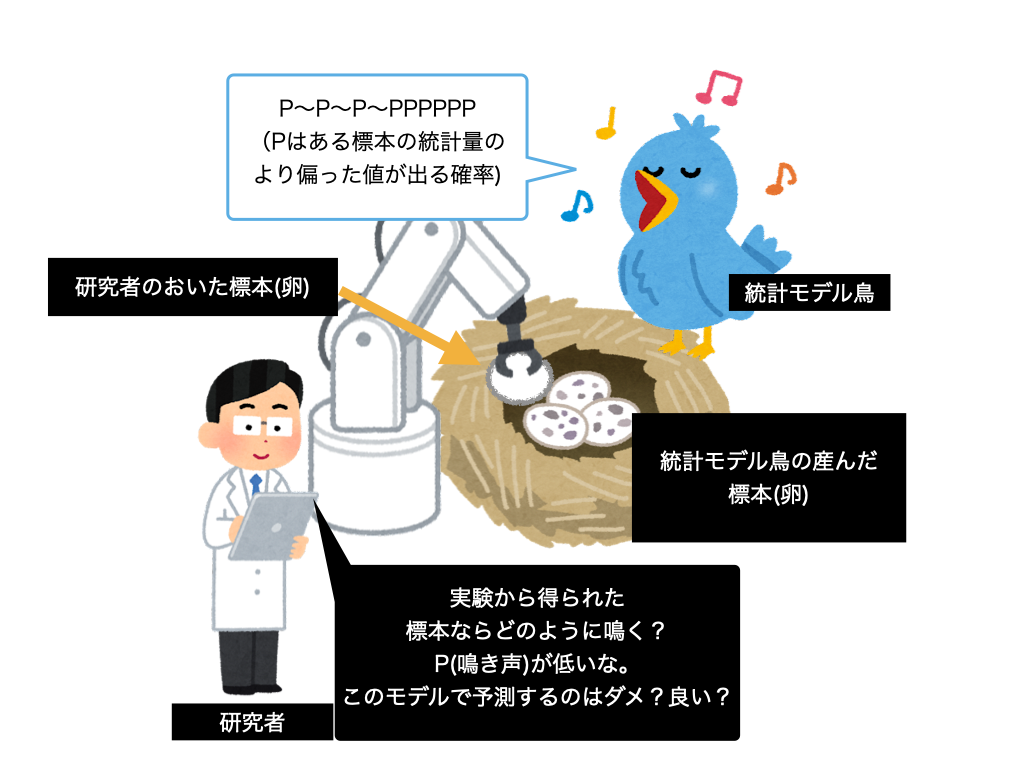
\includegraphics[width=15cm]{./image/01_/conceptual_diagram/conceptual_diagram.003.png}
        \caption{統計量を使ったモデルとデータの比較に関する概念図}
        \label{fig:conceptual_diagram_test}
    \end{center}
\end{figure}
    


\begin{SMbox}{偶然の差が生じたかを確かめたい}
    「偶然の差が生じたかを確かめたい」や「こんなことが起こる確率は$5\%$くらい」という言葉を統計学の教科書で見たことがある。これらは、本書での説明とは異なる前提をもとに議論を進めており、本書と解釈の互換性はない。
    %「統計モデルの上で統計量が現れる確率が十分小さいことを確かめたい」や「統計モデル上でそのような統計量が得られる確率が$5\%$」を省略して書いたものです。
    
    科学では、実験で得られたデータは、同様の実験を行った場合、同様のものが得られるということが前提になっている。このことを現象に再現性があると言う。
    再現性のないデータを現状の統計学で扱うことや、現実の現象が得られる確率を議論することは困難である。

    本書の前提を元にすれば、「こんなこと(これ以上に偏った統計量値)が(モデル内で)起こる確率は$5\%$くらい」ということを省略して「こんなことが起こる確率は$5\%$くらい」と言うことはできる。また、現実において起こりやすいのかどうかについては議論できない。
\end{SMbox}


\subsection{$p$値を使った判断に関する注意}
$p$値を元に統計モデルとデータの不一致を考えるとき、$p$値はモデルとデータの乖離を示す指標の一つであると言うことを意識しなければならない。このことを忘れてしまい、次の間違った判断を行うことがある。
\begin{enumerate}
    \item $p$値が0に近いならば、統計モデルによりデータを予測できないと判断する
    \item $p$値が1に近いならば、統計モデルによりデータを予測できると判断する
\end{enumerate}
それぞれのデータがどのようなものなかのかを確認してみる。
\subsubsection{$p$値が0に近い$\rightarrow$統計モデルによりデータを予測できないと判断}

\subsubsection{$p$値が1に近い$\rightarrow$統計モデルによりデータを予測できると判断}




\section{NP型}
NP型では、すでに前提になっていることから著しく外れたことが起きたことを検出するための方法である。
言い換えるなら、まず、何度も検証を行っていてモデルが事象をよく予測することがわかっている状況を構築する。
そして、その繰り返し事象の中から、いくつかの無作為抽出し、計測を行う。
最後に、計測の平均がモデルの予測を著しく外れているならば、前提に狂いが生じたのではないかと疑う。

\subsection{解決できる問題}
NP型で扱う問題をいくつか挙げる。
\begin{quote}
    ある調味料の製造ラインでは, 砂糖の含有量 (g) は, 原料の不均一や製造ラインの狂いなどから変動するが, 標準偏差は常に一定で$\sigma=3$ の正規分布に従っているとしてよい. 各製品の砂糖の含有量が$\mu=60$になるように調整してラインを稼働させて, しばらくしてから, $25$個の製品を抜取検査したところ, 砂糖の含有量の平均値は$\bar{x}=61.63$であった. その時点で製造ラインは$\mu=60$を保持していると言えるだろうか.

    %\\ https://www.math.is.tohoku.ac.jp/~obata/student/subject/file/2019-EStat-All.pdf
\end{quote}
正規モデル$M(60,3^2)$によって予測ができるという前提条件を満たしている。この前提を元に、無作為抽出した$25$個がそのモデルにより予測できるのかを調べる。標本全体とモデルの累積分布などを比較する方法もあるが、ここでは、検定によって調べてみる。このモデルでは、
\begin{equation*}
    Z=\sqrt{n}\frac{\mu-\bar{x}}{\sigma} \sim N(0,1)
\end{equation*}
である。変数を入れれば、$Z=2.72$となる。$vavrPhi(Z)<\varPhi(1/20=0.05)$であり、モデル内で、20回に1回よりも少ない頻度で観測されないようなことが現実で起きている。
または、$\varPhi(Z)<\varPhi(2\sigma=2)$であり、$2\sigma=2$(標準正規分布の中で)よりも珍しいことが起きているので、モデルでの予測ができないことが起きている。
偶発的に生じた可能性も捨てられないが、製造過程に不具合が生じているのではないかと推測される。




\subsection{解釈}

%NP型の問題では、前提が守られていることを確認できる状況においてのみ使える。
%言い換えれば、何度も何度も繰り返しモデルと現象を比較した結果、モデルが現象をよく予測できるということが確かめられているということである。
%頻度論で明らかになった数学を全て使うことができる。

\section{ハイブリッド型}
\subsection{解決できる問題}



\begin{SMbox}{有意性検定・仮説検定}
    Fisherは、帰無仮説を設定し、帰無仮説とデータを比較検討する方法を構築した。これを、有意性検定という。これに対して、Neyman-Pearsonらは、帰無仮説に加えて、対立仮説を設定し、データを元に帰無仮説を棄却するかの判断を有意水準により行う意思決定の枠組みを構築した。これを、仮説検定と呼ぶことがある\cite{1573106361610039296}。
    現代の科学の多くは、FisherとNeyman-Pearsonの両方を組み合わせ、帰無仮説・対立仮説を設定し、帰無仮説とデータの乖離を$p$値によって調べ、棄却するかを検討する。ここでの$p$値は、Neyman-Pearsonの解釈から、20回に1回程度のことを有意と呼ぶことにしている。
    この流派をハイブリッド仮説検定法\cite{published_papers/18436201}と呼ぶことにする。
        %有意性検定を統計学\cite{upton2010統計学辞典,2009数理統計ハンドブック}や数学\cite{日本数学会2007岩波数学辞典}の辞書で調べたが、該当する言葉は見つからなかった。一方で、仮説検定は統計学\cite{upton2010統計学辞典,2009数理統計ハンドブック}などの辞書でも見つけることができた。
        %この言葉の使い方は、\cite{鳥類学における統計学_2018}に乗っていた。
\end{SMbox}


%\chapter{モデルを使った有意性検定}

\section{モデルの設定}
帰無仮説$\mu=\mu_0$をを含む統計モデル$M(\mu_0)$を帰無モデル($M_{H_0}$)、対立仮説$\mu\neq \mu_0$を含む統計モデル$M(\mu\neq\mu_0)$を対立モデル($M_{H_1}$)と呼ぶ。
一般に、統計モデルの否定したい母数$\mu_0$を帰無仮説と言い、その母数ではないという$\mu\neq\mu_0$を対立かせつと言います。つまり、次のように帰無仮説を含む統計モデル$M_0$を構築します。

具体的には、データがある特定の母数$\mu$をもつ統計モデルの信頼区間に含まれるか否かによって、統計モデルが棄却されるかを調べます。
\begin{itemize}
    \item i.i.d
    \item 数学関数
    \item 統計モデルの母数を$\mu$とし、$\mu=\mu_0$
\end{itemize}
一番最後の仮説が帰無仮説と言います。
対立仮説を含む統計モデル$M_1$は、$M_0$と同様の仮説(1),(2)から構成されますが、仮説3は統計モデル$M_0$と$M_1$で異なります。
\begin{itemize}
    \item i.i.d
    \item 数学関数
    \item 統計モデルの母数を$\mu$とし、$\mu\neq\mu_0$
\end{itemize}
一番最後の仮説が対立仮説です。$M_1$の最後の仮説は、$M_0$の最後の仮説の否定系になります。

二つの統計モデルを作って、$M_0$で計算される信頼区間に、データから得られる統計量が入らないなら、$M_0$は棄却されます。逆に、統計量が信頼区間に入るなら、何も起こりません。
このように、否定したい仮説を設定し、少なくとも帰無仮説を含む統計モデルはだめだったと判断します。

